\documentclass[12pt]{article}
\usepackage{amsmath,amssymb,amsfonts}
\usepackage{graphicx}
\usepackage{geometry}
\geometry{margin=1in}

\title{Beyond Utilization-Based Curves. Trade-Specific Interest Rate Models}
\author{}
\date{}

\begin{document}

\maketitle

\begin{abstract}
% Abstract will be added in the final stage.
\end{abstract}

% Context and key points for the introduction will be inserted here.
\section{Introduction}

Interest rate models within credit protocols play a crucial role in balancing supply and demand for funds. These models are fundamental for optimal interest rate discovery and ensuring that liquidity pools remain both solvent and liquid. By using the utilization rate as a key factor, these models dynamically estimate current supply and demand levels, which in turn incentivizes lending and borrowing activities.

One widely adopted approach is the kinked utilization-based interest rate curve. In this model, the interest rate \( r(u) \) is defined as a piecewise function of the utilization rate \( u \). The formula is given by:
\[
r(u) = 
\begin{cases} 
r_{\text{base}} + r_{\text{slope1}} \cdot u, & \text{if } u \leq u^* \\
r_{\text{base}} + r_{\text{slope1}} \cdot u^* + r_{\text{slope2}} \cdot (u - u^*), & \text{if } u > u^*
\end{cases}
\]
Here, \( r_{\text{base}} \) denotes the base interest rate, \( r_{\text{slope1}} \) and \( r_{\text{slope2}} \) represent the interest rate slopes before and after the kink point respectively, and \( u^* \) is the critical utilization threshold where the curve shifts. This formulation is designed to adjust rates effectively as utilization changes, providing a clear signal to both lenders and borrowers.

The success of utilization-based curves is demonstrated by platforms like AAVE, which has reached over \$20B in Total Value Locked (TVL), and Morpho, with a TVL of around \$5B. Despite these achievements, there remain significant issues with utilization-based curves. While retail traders appreciate the simplicity of these models, they often lack the sophistication required by institutional DeFi hedge funds. These institutions face unique challenges that demand more advanced interest rate frameworks, prompting the exploration of trade-specific models that can better address complex market dynamics.


\section{Caveats of Utilization-Based Curves}

Utilization-based interest rate models, despite their widespread adoption in DeFi protocols, are burdened by several critical issues. One of the most prominent drawbacks is the inherent lack of predictability and stability. This issue becomes especially acute as DeFi hedge funds begin participating in complex strategies such as leveraging and looping. When these institutional players enter the market, they are quickly joined by other market participants—including retail users—who crowd into the same trade opportunities. As a direct consequence of this crowding, the expected return from a leveraged trade can drop precipitously or even turn negative, undermining the original rationale for engaging in such strategies.


In practical terms, this volatility forces funds to remain in a state of constant vigilance. They must continuously monitor the difference between the prevailing borrow rate and the yield generated by their leveraged positions. Moreover, these funds have to track the pool's utilization in real time, as any shift in utilization can drastically alter the lending and borrowing rates. Such monitoring is not limited to the initiation of trades; funds must also carefully project the potential impact on interest rates should they decide to enter or exit a pool, making the entire process both resource-intensive and fraught with risk.


This unpredictability further compels hedge funds to adopt sophisticated analytical frameworks. In particular, they are driven to analyze the behavior of other market participants from a game theory perspective. By attempting to anticipate how various traders might act—especially under rapidly changing market conditions—hedge funds strive to understand the potential impact on the overall utilization rate. This deep analysis of market behavior is one of the principal reasons why many DeFi hedge funds prefer to secure fixed interest rate loans from prime brokers. Fixed-rate loans provide a more predictable trading environment, effectively insulating them from the erratic fluctuations that characterize utilization-based curves.

The problem of volatility in utilization and the resulting fluctuations in lending and borrowing Annual Percentage Yields (APY) affects both borrowers and lenders. On one side, borrowers are forced to contend with a market where the net expected returns can swing wildly, potentially pushing them into negative territory. On the other side, lenders—who ideally seek a smooth and predictable APY for their lending operations—are not spared from these disturbances. The constant changes in market conditions create an environment where neither party can confidently plan their financial strategies.

Empirical observations at Arkis illustrate this imbalance quite starkly. Although borrowers struggle with the challenges posed by ever-changing utilization levels, they are often able to achieve high yields through looping activities, sometimes generating APYs of 30\% or even exceeding 50\%. In contrast, lenders generally receive far more modest returns, typically in the range of 9\% to 12\% on most blue-chip lending protocols. This disparity leaves lenders as the least rewarded participants in the DeFi ecosystem, further highlighting the need for a more balanced approach.

All the issues discussed above point to the necessity for an improved interest rate model—one that can overcome the limitations of current utilization-based curves. Such a model should embody the following properties:
\begin{itemize}
    \item It must take into account the borrower’s expected return to ensure that they are not forced into trades with a negative net expected value.
    \item It should provide stable lending and borrowing APY, thereby reducing the uncertainty and volatility that currently afflicts market participants.
    \item It must maintain a stable and high utilization level (ideally between 80\% and 90\%) while simultaneously offering enhanced rewards to liquidity providers.
\end{itemize}

\section{Methodology}

In this section, we describe how the paper is organized and detail the research methodology. The primary goal is to model the lending/borrowing environment in DeFi by employing two complementary simulation techniques:
\begin{enumerate}
    \item \textbf{Stochastic simulations} of lenders' and borrowers' behavior.
    \item \textbf{Time series simulations} of the expected return of yield assets.
\end{enumerate}
These approaches allow us to capture both the probabilistic nature of market participant actions and the dynamic evolution of yield returns over time.

\subsection{Assumptions for Lenders}

Based on multiple interviews with Arkis' institutional lenders, we incorporate the following assumptions for modeling lender behavior:
\begin{itemize}
    \item Lenders' deposits and withdrawals are modeled as normally distributed random variables:
    \[
    D \sim \mathcal{N}(\mu_{\text{deposit}}, \sigma_{\text{deposit}}^2), \quad W \sim \mathcal{N}(\mu_{\text{withdraw}}, \sigma_{\text{withdraw}}^2)
    \]
    where \(D\) denotes deposits and \(W\) withdrawals.
    \item When the lending APY is greater than or equal to a \emph{desired} threshold, \(\text{desired\_APY}\), there is a probability \(p_{\text{desired}}\) that lenders will deposit funds. We assume that \text{desired\_APY}\ is \bold{20\%} while \(p_{\text{desired}}\) is \bold{80\%}.
    \item Conversely, if the lending APY is less than or equal to an \emph{undesired} threshold, \(\text{undesired\_APY}\), there is a probability \(p_{\text{undesired}}\) that lenders will withdraw funds (i.e., record a negative deposit). In our simulations \text{undesired\_APY}\ is \bold{10\%} while \(p_{\text{undesired}}\) is \bold{80\%}.
    \item If the lending APY lies between \(\text{undesired\_APY}\) and \(\text{desired\_APY}\), there is a 50\% probability that a lender will either deposit or withdraw funds.
\end{itemize}
These assumptions encapsulate the idea that lenders maintain a minimum hurdle rate (\(\text{undesired\_APY}\)) for their investments. When the APY is high (i.e., reaches \(\text{desired\_APY}\)), lenders are more inclined to allocate capital to the protocol.

\subsection{Assumptions for Borrowers}

For borrowers, our model is based on the following assumptions:
\begin{itemize}
    \item If the spread between the expected return on a yield asset and the current borrow rate is negative (i.e., yielding a negative expected value), there is a 90\% probability that the trader will close their position and withdraw from the pool.
    \item If the spread is positive, the probability of holding the position is uniformly distributed in the interval 
    \[
    \left[0, \max\left(1, \text{spread} \times 10\right)\right].
    \]
    For instance, a 5\% spread corresponds to a 50\% chance of holding the trade, while a 9\% spread results in a 90\% probability.
    \item The probability of a new trader entering the trade is modeled using an exponential function defined by two parameters (steepness and shift). The function is expressed as:
    \[
    P(\text{borrow more} \mid r_{\text{exp}}) = \frac{1}{1 + e^{-a (r_{\text{exp}} - b)}},
    \]
    where \(a = 90.2\) and \(b = 0.05\), and \(r_{\text{exp}}\) denotes the spread between expected return and borrow rate.
\end{itemize}


\begin{figure}[h!]
\centering
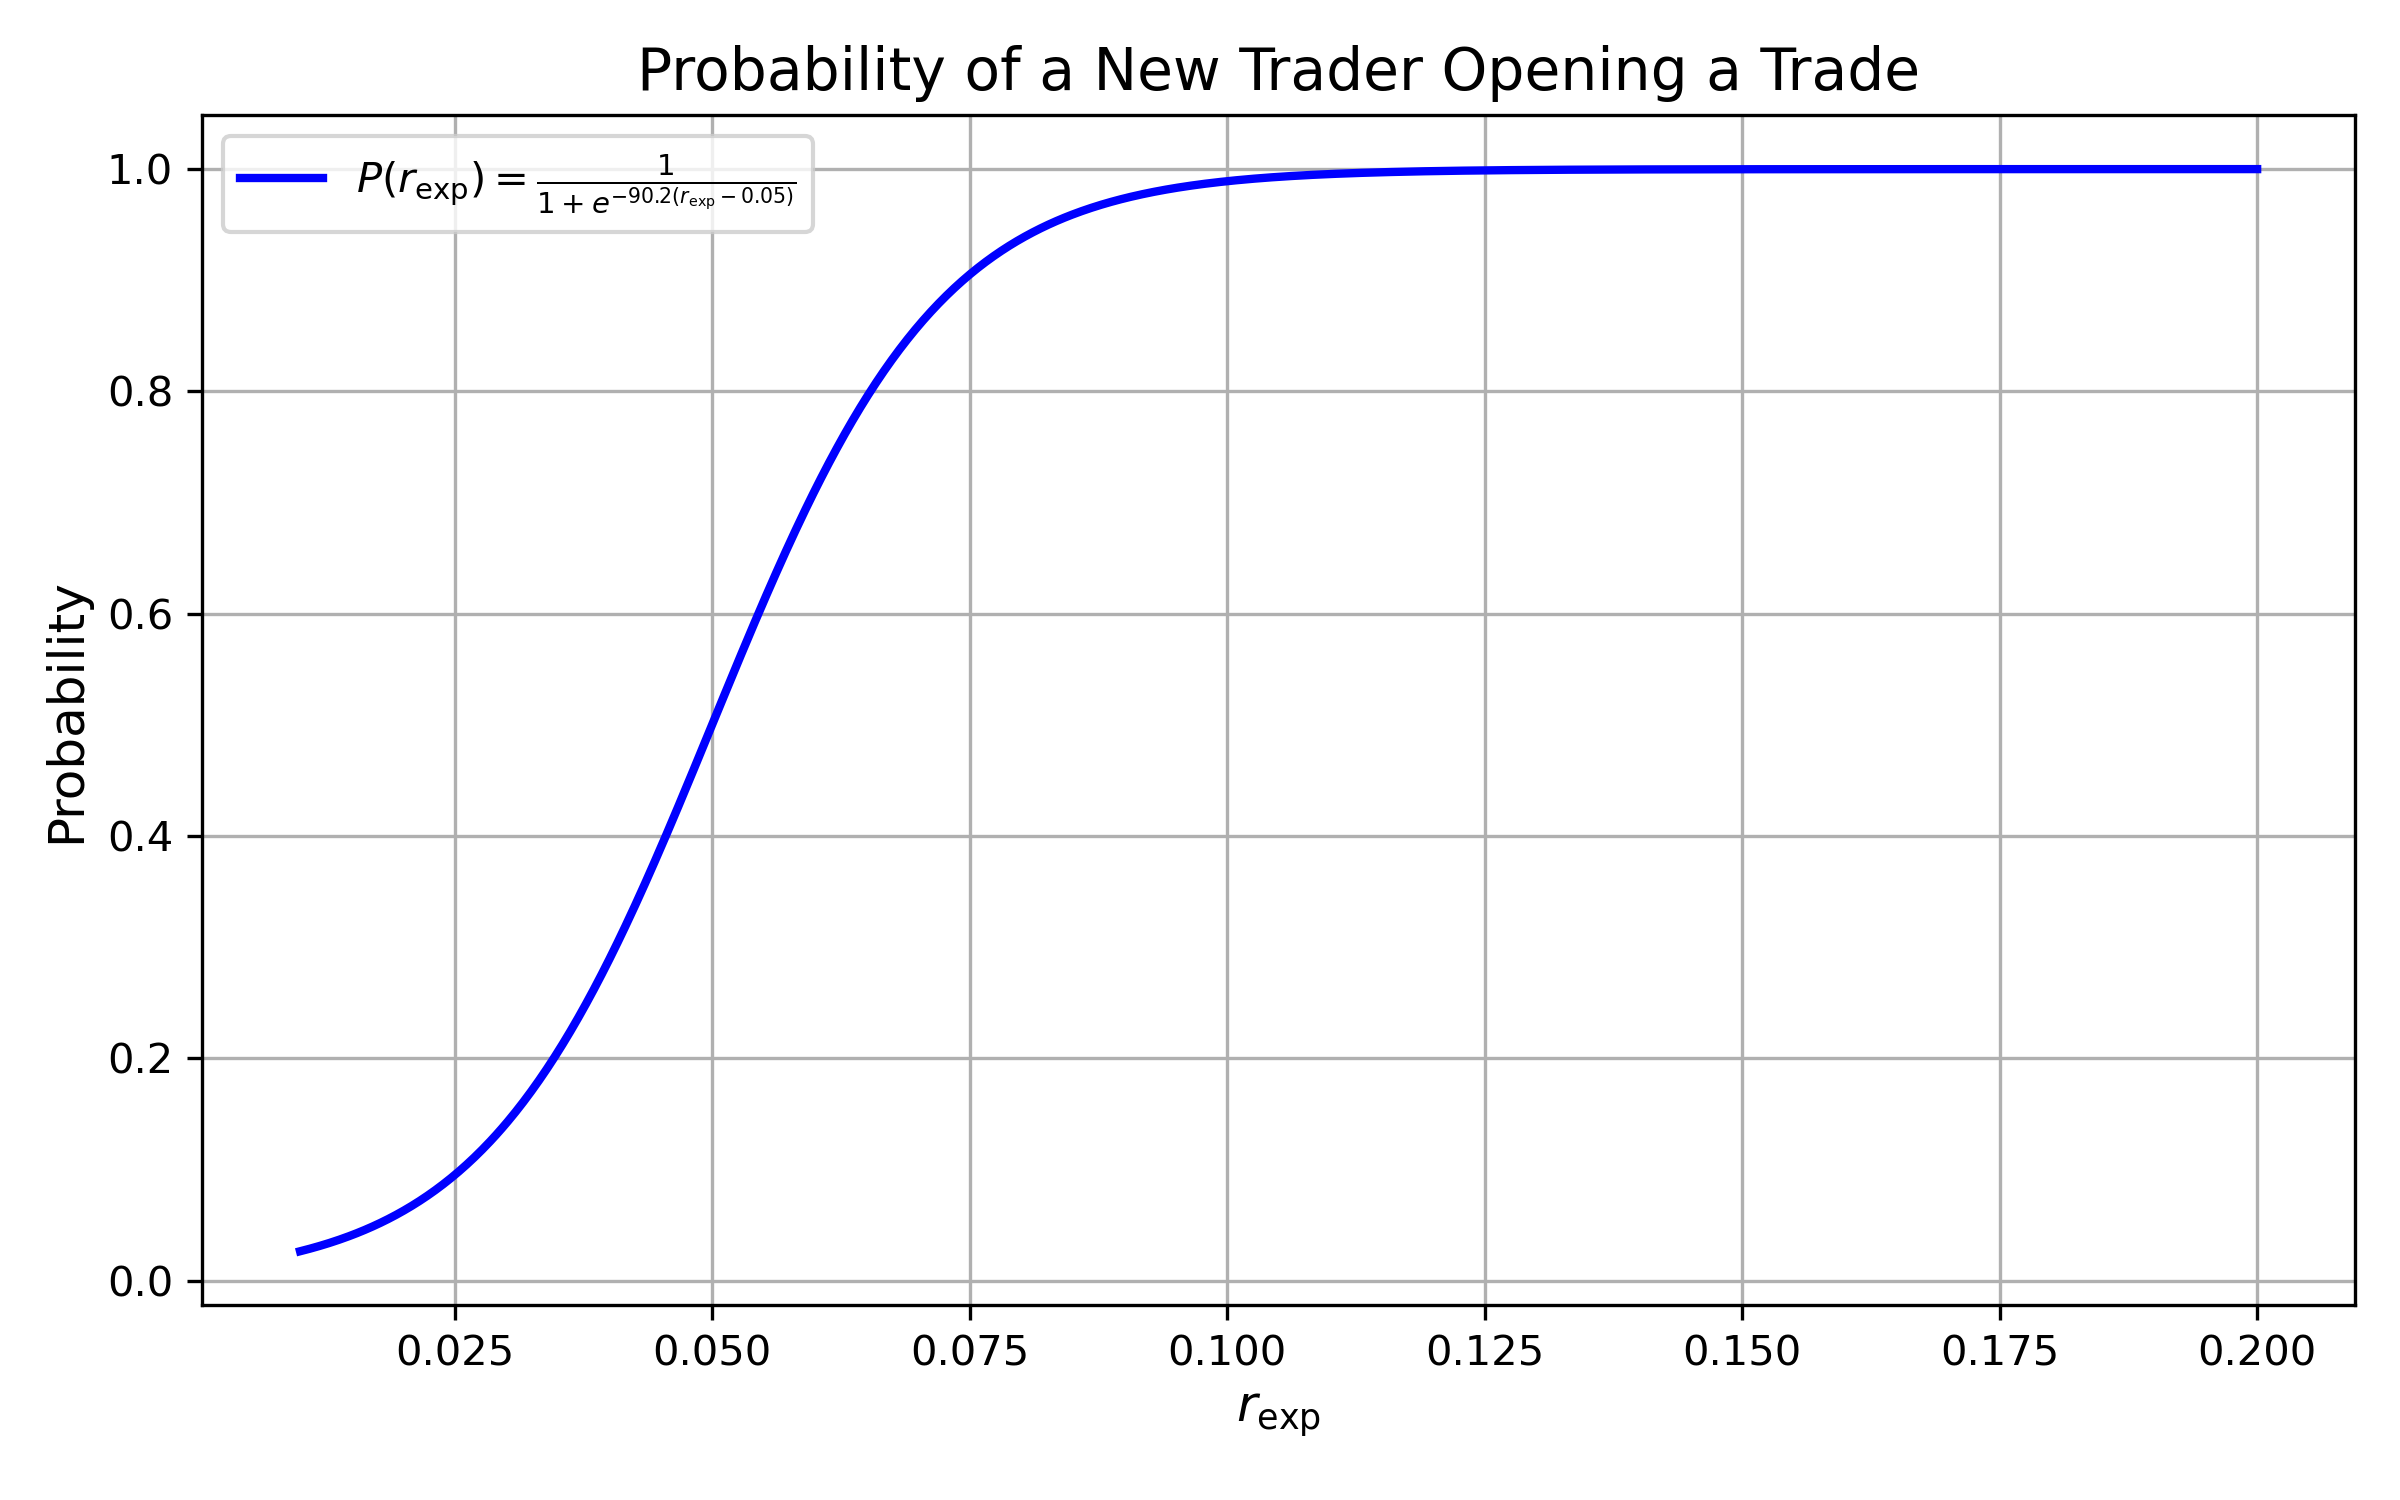
\includegraphics[width=0.8\textwidth]{images/prob_borrow_more.png}
\caption{Probability of a new trader opening trade as a function of the spread \(r_{\text{exp}}\).}
\label{fig:prob_borrow_more}
\end{figure}



\subsection{Summary of Methodology}

In summary, our methodology integrates stochastic simulations of market participant behavior with time series simulations of yield asset returns. The assumptions outlined above, derived from extensive interviews with institutional lenders and borrowers at Arkis, form the backbone of our simulation framework. These assumptions enable us to capture key dynamics, such as:
\begin{itemize}
    \item The dependency of lender behavior on lending APY relative to desired and undesired thresholds.
    \item The nuanced decision-making process of borrowers based on the spread between expected returns and current borrow rates.
    \item The exponential probability model governing the entry of new traders.
\end{itemize}

The idea of the paper is to construct various interest rate models based on specifics of widely adopted trades in DeFi (carry, Pendle PT/LP loop), run simulations using the assumptions above, and analyze the following characteristics in comparison with the utilization-based curve: 
\begin{itemize}
	\item Total Lending APY earned by liquidity providers taking into account pool utilization. 
	\item Pool utilization and its stability (t-value). 
	\item Distribution of total traders' performance considering a maximum of x3 leverage. 
	\item Contribution to traders' performance from leveraging activities. 
\end{itemize}






% Additional sections can be added following the same structure.

\end{document}
